\setcounter{chapter}{9} 
\chapter*{Chapter (9): Mobile Application}
\addcontentsline{toc}{chapter}{Chapter (9): Mobile Application} 
\renewcommand{\thesection}{\thechapter.\arabic{section}}
\setcounter{section}{0}
\captionsetup[figure]{justification=centering}

\section{Chapter Preview}
This chapter presents the design and features of the caregiver-focused mobile application. It outlines the NativeWind-styled React Native and Expo framework selection, details the biometric telemetry stream and Telegram-based emergency alerts, and explains the remote smart-home and diagnostic control interfaces.

Usability is the core focus of the mobile interface. Caregivers must be able to quickly read critical physiological data and check system alerts with minimal latency. High-contrast indicators and a clear visual hierarchy are implemented to make operation reliable under stress or in low-visibility environments. Table \ref{tab:mobile-requirements} lists the primary functional and non-functional requirements of the mobile app.

\begin{table}[H]
\centering
\caption{Mobile Application Functional and Non-Functional Requirements}
\label{tab:mobile-requirements}
\begin{tabularx}{\textwidth}{|l|>{\raggedright\arraybackslash}X|c|}
\hline
\textbf{Req. ID} & \textbf{Requirement Description} & \textbf{Priority} \\ \hline
FR-01 & Authenticate caregivers and securely link their accounts to the patient's Telegram session. & Must \\ \hline
FR-02 & Monitor patient biometrics (temperature and heart rate) in real time. & Must \\ \hline
FR-03 & Trigger automatic alert notifications to designated Telegram chats during biometric emergencies. & Must \\ \hline
FR-04 & Control smart home devices in the patient's environment (lights, dimmers, locks). & Should \\ \hline
FR-05 & Monitor system diagnostics (battery state, speed limits, controller CPU temperature). & Should \\ \hline
NFR-01 & Minimize latency: Notification transmission delay must remain under 100 ms. & Must \\ \hline
NFR-02 & Accessibility: Support screen readers and high-contrast styling. & Should \\ \hline
NFR-03 & Interface flexibility: Provide dark and light modes for different environment illumination. & Should \\ \hline
\end{tabularx}
\end{table}

\begin{figure}[H]
\centering
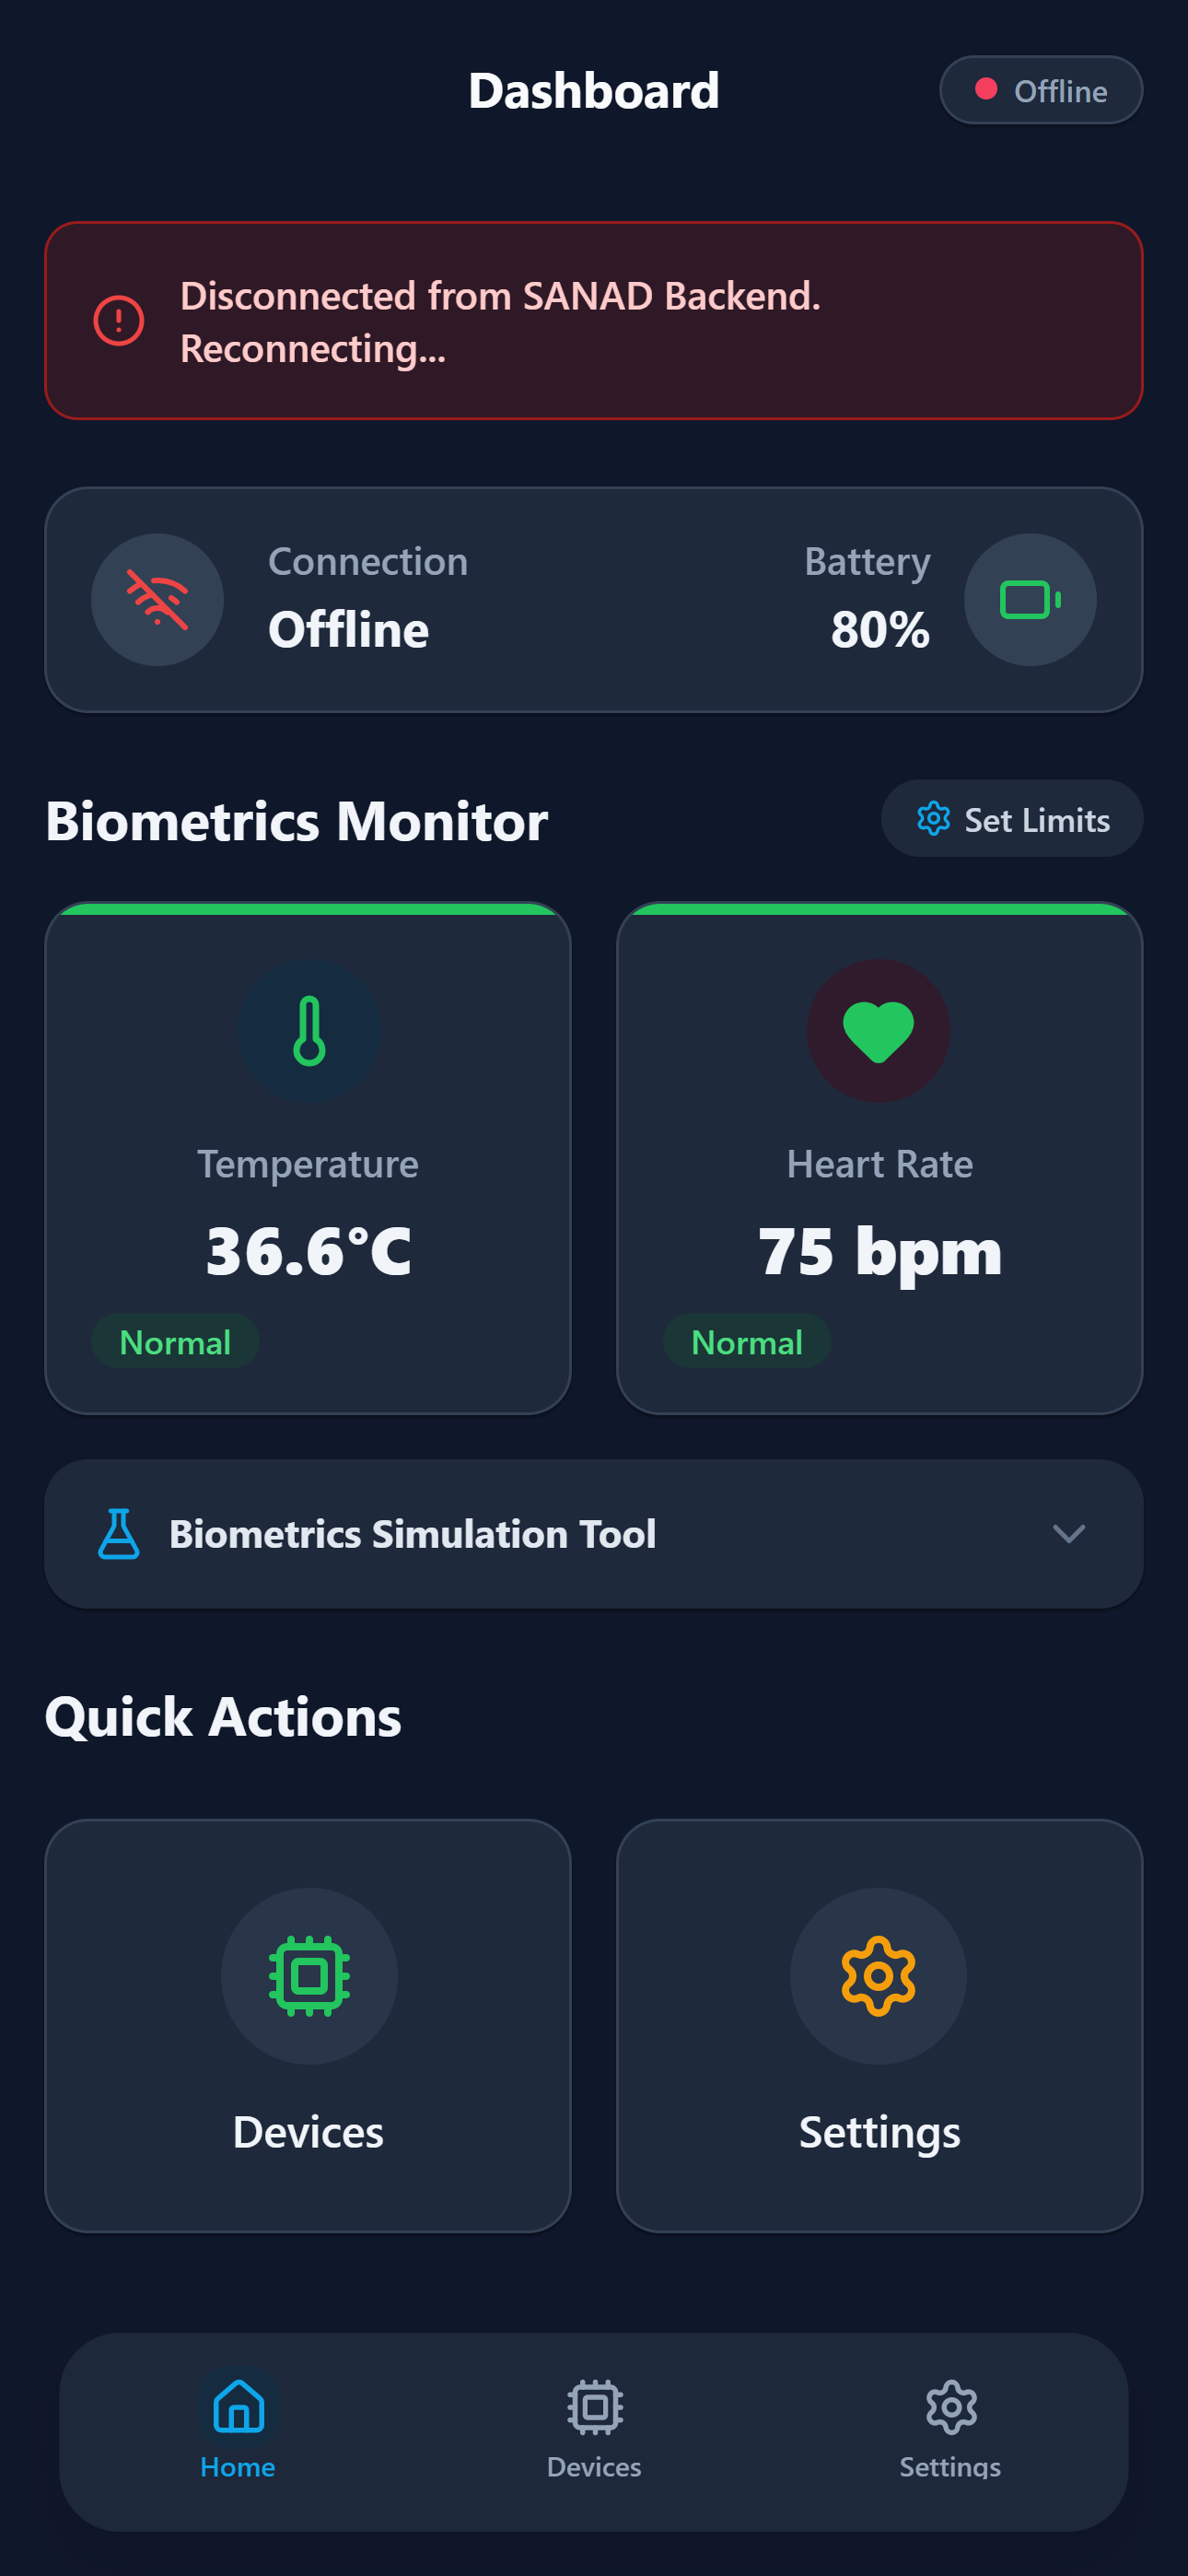
\includegraphics[width=0.45\textwidth]{figures/ch09/mobile_overview.png}
\caption{Main dashboard view of the SANAD mobile application showing active telemetry and biometrics status.}
\label{fig:mobile-overview}
\end{figure}

\section{Technology Stack \& Native Alternatives}
To target both Android and iOS devices from a single codebase, a cross-platform mobile framework was necessary. During the initial design, multiple options were evaluated, including native development, Flutter, progressive web applications (PWAs), and React Native.

\textbf{React Native} was chosen, utilizing the \textbf{Expo} framework (version 54) and \textbf{TypeScript}. React Native compiles to native platform components, ensuring smooth rendering performance and native responsiveness, unlike hybrid WebView-based alternatives. Expo simplifies access to device hardware and provides a clean development workflow. \textbf{NativeWind 4} is used for styling, bringing Tailwind's utility-first class model to React Native.

Table \ref{tab:mobile-frameworks} compares the evaluated mobile frameworks.

\begin{table}[H]
\centering
\caption{Mobile Framework Evaluation Metrics}
\label{tab:mobile-frameworks}
\begin{tabularx}{\textwidth}{|>{\raggedright\arraybackslash}X|c|c|c|}
\hline
\textbf{Metric} & \textbf{React Native (Expo)} & \textbf{Flutter} & \textbf{PWA / WebView} \\ \hline
Development Velocity & Very High & High & High \\ \hline
Code Reusability & > 90\% & > 90\% & 100\% \\ \hline
Bundle Size (Base) & \textasciitilde 22 MB & \textasciitilde 15 MB & < 2 MB \\ \hline
Haptics API Access & Native Wrapper & Native Wrapper & Limited \\ \hline
Layout Engine & Yoga (Flexbox) & Skia Canvas & HTML DOM \\ \hline
\end{tabularx}
\end{table}

Key dependencies in the mobile project include:
\begin{itemize}
    \item \textbf{socket.io-client}: Manages the persistent WebSocket connection to the Node.js server for real-time telemetry.
    \item \textbf{react-native-gesture-handler} \& \textbf{react-native-reanimated}: Powers the interactive elements, such as slide-up panels and smooth drawer transitions.
    \item \textbf{expo-haptics}: Provides physical haptic feedback during alert and emergency events.
    \item \textbf{react-native-toast-message}: Displays overlay notifications for system warnings and connection status changes.
\end{itemize}

\section{Application Architecture \& Routing}
The mobile application uses the \textbf{group-by-feature} directory structure to keep related code modules organized.
The navigation structure is powered by \textbf{Expo Router}. The root layout (\texttt{app/\_layout.tsx}) initializes global connection contexts and checks the user's authentication state. If the user is unauthenticated, they are redirected to the login screen. Once logged in, the app loads the tab navigator (\texttt{app/(tabs)/\_layout.tsx}), which configures the bottom navigation bar and displays the server connection status (Connected/Offline) in the top-right header.


\section{Mobile-to-Server Communication Architecture}
The SANAD mobile application operates as a remote HMI (Human-Machine Interface) for caregivers and medical personnel. To support seamless remote observation, the mobile application establishes two distinct communication channels with the Node.js server. This architecture separates high-frequency telemetry from transactional controls, preventing connection congestion and ensuring that physiological alerts are dispatched and received with sub-second latencies.

\subsection{Communication Topology}
The networking layout of the mobile monitoring system is divided into the client-side presentation layer (React Native mobile application and Telegram client), the supervisory layer (Node.js server), and the execution layer (onboard ROS 2 bridge and smart home appliances). Figure \ref{fig:mobile-server-comm-tikz} shows the network topology and the specific protocol pathways connecting these subsystems.

\begin{figure}[H]
\centering
\begin{tikzpicture}[
    font=\sffamily\small,
    node distance=2.2cm and 2.5cm,
    clientNode/.style={rectangle, draw=blue!70!black, fill=blue!10, rounded corners, minimum width=3.5cm, minimum height=1.2cm, align=center, thick, drop shadow},
    serverNode/.style={rectangle, draw=orange!80!black, fill=orange!10, rounded corners, minimum width=3.5cm, minimum height=1.2cm, align=center, thick, drop shadow},
    hardwareNode/.style={rectangle, draw=green!60!black, fill=green!10, rounded corners, minimum width=3.5cm, minimum height=1.2cm, align=center, thick, drop shadow},
    telegramNode/.style={rectangle, draw=cyan!70!black, fill=cyan!10, rounded corners, minimum width=3.5cm, minimum height=1.2cm, align=center, thick, drop shadow},
    iotNode/.style={rectangle, draw=purple!70!black, fill=purple!10, rounded corners, minimum width=3.5cm, minimum height=1.2cm, align=center, thick, drop shadow},
    httpArrow/.style={Latex-Latex, draw=red!70!black, thick},
    wsArrow/.style={Latex-Latex, draw=teal!70!black, dashed, thick},
    apiArrow/.style={-Latex, draw=cyan!80!black, thick},
    rosArrow/.style={Latex-Latex, draw=green!60!black, thick}
]

    \node[clientNode] (mobile) {Caregiver Mobile App\\(React Native / Expo)};
    
    \node[serverNode, right=of mobile, yshift=1cm] (nodejs) {Node.js Server\\(REST API \& JWT)};
    \node[serverNode, right=of mobile, yshift=-1cm] (socketio) {Socket.io Gateway\\(Real-time Streams)};
    
    \node[telegramNode, above=of nodejs] (tgBot) {Telegram Bot API\\(Telegram Servers)};
    \node[clientNode, left=of tgBot] (tgClient) {Caregiver Telegram\\(Client App)};
    
    \node[hardwareNode, right=of socketio] (rosbridge) {ROS 2 Bridge\\(rosbridge\_server)};
    \node[iotNode, right=of nodejs] (iot) {Smart Home Devices\\(IoT Controller)};

    \begin{scope}[on background layer]
        \node[draw=orange!60, fill=orange!5, dotted, thick, rounded corners, fit=(nodejs) (socketio), label={[orange!80!black]right:Node.js Server Backend}] (serverGroup) {};
    \end{scope}

    \draw[httpArrow] (mobile) -- node[above, sloped, font=\tiny] {HTTPS (JWT / OTP)} (nodejs);
    \draw[wsArrow] (mobile) -- node[below, sloped, font=\tiny] {Socket.io Persistent} (socketio);
    
    \draw[apiArrow] (nodejs) -- node[left, font=\tiny] {HTTPS Bot API} (tgBot);
    \draw[apiArrow] (tgBot) -- node[above, font=\tiny] {Alerts} (tgClient);
    
    \draw[rosArrow] (socketio) -- node[above, font=\tiny] {JSON over WS} (rosbridge);
    \draw[apiArrow] (nodejs) -- node[above, font=\tiny] {UDP / HTTP} (iot);

\end{tikzpicture}
\caption{Communication topology of the mobile monitoring system, showing REST and Socket.io transport channels between the React Native client, Node.js server, Telegram services, and ROS 2 execution stack.}
\label{fig:mobile-server-comm-tikz}
\end{figure}

\subsection{REST API and Stateless Interventions}
Stateless and transactional operations are handled through standard HTTPS request-response cycles. These transactions include caregiver registration and authentication, generation and validation of Telegram session tokens, smart home device network discovery queries, and profile configuration adjustments. In compliance with security standards, all transactional endpoints are protected by JSON Web Token (JWT) verification, requiring the client to pass the bearer token in the HTTP Authorization header. This channel is also subject to strict schema validation on the backend to filter out malformed requests before they trigger database queries.

\subsection{Socket.io persistent Telemetry Channel}
For streaming real-time biometric diagnostics and system health updates, the mobile application maintains a persistent connection via the Socket.io protocol (a layer built on top of TCP WebSockets). This persistent, full-duplex socket allows the Node.js server to push new biometric metrics (heart rate, body temperature) and diagnostic values (onboard CPU temperature, speed limit modifiers, battery percentages) to the client as soon as they are received from the ROS 2 bridge. This architecture eliminates the processing and network overhead of traditional HTTP polling, ensuring that the caregiver's dashboard displays real-time patient states.

\subsection{ROS-to-Web Message Mapping}
The Node.js server functions as a message aggregator and translator. It maintains a persistent WebSocket connection to the onboard \texttt{rosbridge\_server}, subscribing to native ROS 2 topics and publishing commands. When ROS 2 messages are received, the server extracts the raw payload values and maps them directly to corresponding Socket.io events. To guarantee type compatibility, the mobile client connection provider translates raw socket JSON responses into standardized ROS message schemas, such as representing coordinates as a ROS \texttt{PoseWithCovarianceStamped} structure before passing them to client-side callback hooks.

\subsection{Connection Resiliency and Heartbeats}
To handle network disruptions, the mobile application integrates a connection provider that manages socket state lifecycles:
\begin{itemize}
    \item \textbf{Heartbeat Loop}: The mobile client exchanges periodic keep-alive ping-pong packages with the Node.js gateway. If no response is received within $2500\text{ ms}$, the connection is marked as disconnected.
    \item \textbf{Visual Notification}: The application displays a warning banner and changes the status indicator in the tab header to "Offline" to alert the caregiver.
    \item \textbf{Exponential Reconnection}: The client automatically attempts to re-establish the Socket.io connection using an exponential backoff algorithm (reconnecting every $5\text{ seconds}$ initially, and scaling up to $30\text{ seconds}$ to conserve mobile battery).
    \item \textbf{Local Cache Persistency}: While disconnected, the application caches local parameters (such as the last targeted Telegram chat ID and base connection URLs) in local persistent storage, restoring the client to a functional state immediately once connectivity is re-established.
\end{itemize}


\section{Biometrics Monitor \& Alarm Pipeline}
Patient safety is a key priority for the SANAD system. The mobile application features a real-time \textbf{Biometrics Monitor} (\texttt{HomeScreen}) that tracks the patient's body temperature and heart rate.

\subsection{Metrics Processing \& Fluctuation}
In the current implementation, biometric telemetry is processed in real time. To account for live physiological changes, a background timer in the \texttt{useBiometrics.ts} hook fluctuates values every 3 seconds:
\begin{align}
T_{t+1} &= T_t + \delta_T - 0.15 \cdot (T_t - T_{\text{baseline}}) \\
\text{HR}_{t+1} &= \text{HR}_t + \delta_{\text{HR}} - 0.15 \cdot (\text{HR}_t - \text{HR}_{\text{baseline}})
\end{align}
where $T_{\text{baseline}} = 36.6^{\circ}\text{C}$ and $\text{HR}_{\text{baseline}} = 75\text{ bpm}$. The random steps $\delta_T \in [-0.06, 0.06]$ and $\delta_{\text{HR}} \in [-1, 1]$ represent natural variations, while the proportional feedback term pulls the metrics back toward the baseline to prevent drift.

\subsection{Threshold Alarms}
Caregivers can set custom safety ranges for the patient's biometrics using slider controls:
\begin{itemize}
    \item \textbf{Temperature Limits}: Min temperature ($34.5^{\circ}\text{C} \dots 36.5^{\circ}\text{C}$), Max temperature ($37.0^{\circ}\text{C} \dots 39.0^{\circ}\text{C}$).
    \item \textbf{Heart Rate Limits}: Min heart rate ($40 \dots 75\text{ bpm}$), Max heart rate ($85 \dots 130\text{ bpm}$).
\end{itemize}

If a patient's metrics cross these thresholds, the state machine triggers an emergency alert. The app displays a local warning banner, sends a system notification, and dispatches an alert message to the caregiver's Telegram account. When the metrics return to normal, the system automatically sends a resolution update, keeping the caregiver informed.

\begin{figure}[H]
\centering
\begin{tikzpicture}[
    font=\sffamily\small,
    node distance=2.2cm and 2.5cm,
    state/.style={circle, draw=blue!70!black, fill=blue!10, thick, minimum size=2.2cm, align=center, drop shadow},
    activeState/.style={circle, draw=red!80!black, fill=red!10, thick, minimum size=2.2cm, align=center, double, drop shadow},
    arrow/.style={-Latex, thick, draw=gray!80},
    transLabel/.style={font=\tiny, fill=white, align=center}
]

    % States
    \node[state] (normal) {Normal\\(Monitoring)};
    \node[state, right=of normal] (breach) {Breach\\Detected};
    \node[activeState, below=of breach] (alarm) {Alarm Active\\(Alert Sent)};
    \node[state, below=of normal] (resolve) {Vitals\\Restored};

    % Transitions
    \draw[arrow] (normal) -- node[above, transLabel] {Vitals Exceed\\Limits} (breach);
    \draw[arrow] (breach) -- node[right, transLabel] {Persistent Breach\\(Trigger Timer)} (alarm);
    
    % Breach to Normal (False alarm / transient)
    \draw[arrow, bend right=30] (breach) to node[below, transLabel] {Vitals Recover\\Immediately} (normal);
    
    % Alarm to Resolve
    \draw[arrow] (alarm) -- node[below, transLabel] {Vitals Return\\to Normal} (resolve);
    
    % Resolve to Normal
    \draw[arrow] (resolve) -- node[left, transLabel] {Send Resolution\\Message} (normal);

\end{tikzpicture}
\caption{State machine diagram illustrating the biometrics monitor alarm pipeline lifecycle.}
\label{fig:biometrics-alarm-state-machine}
\end{figure}

\begin{figure}[H]
\centering
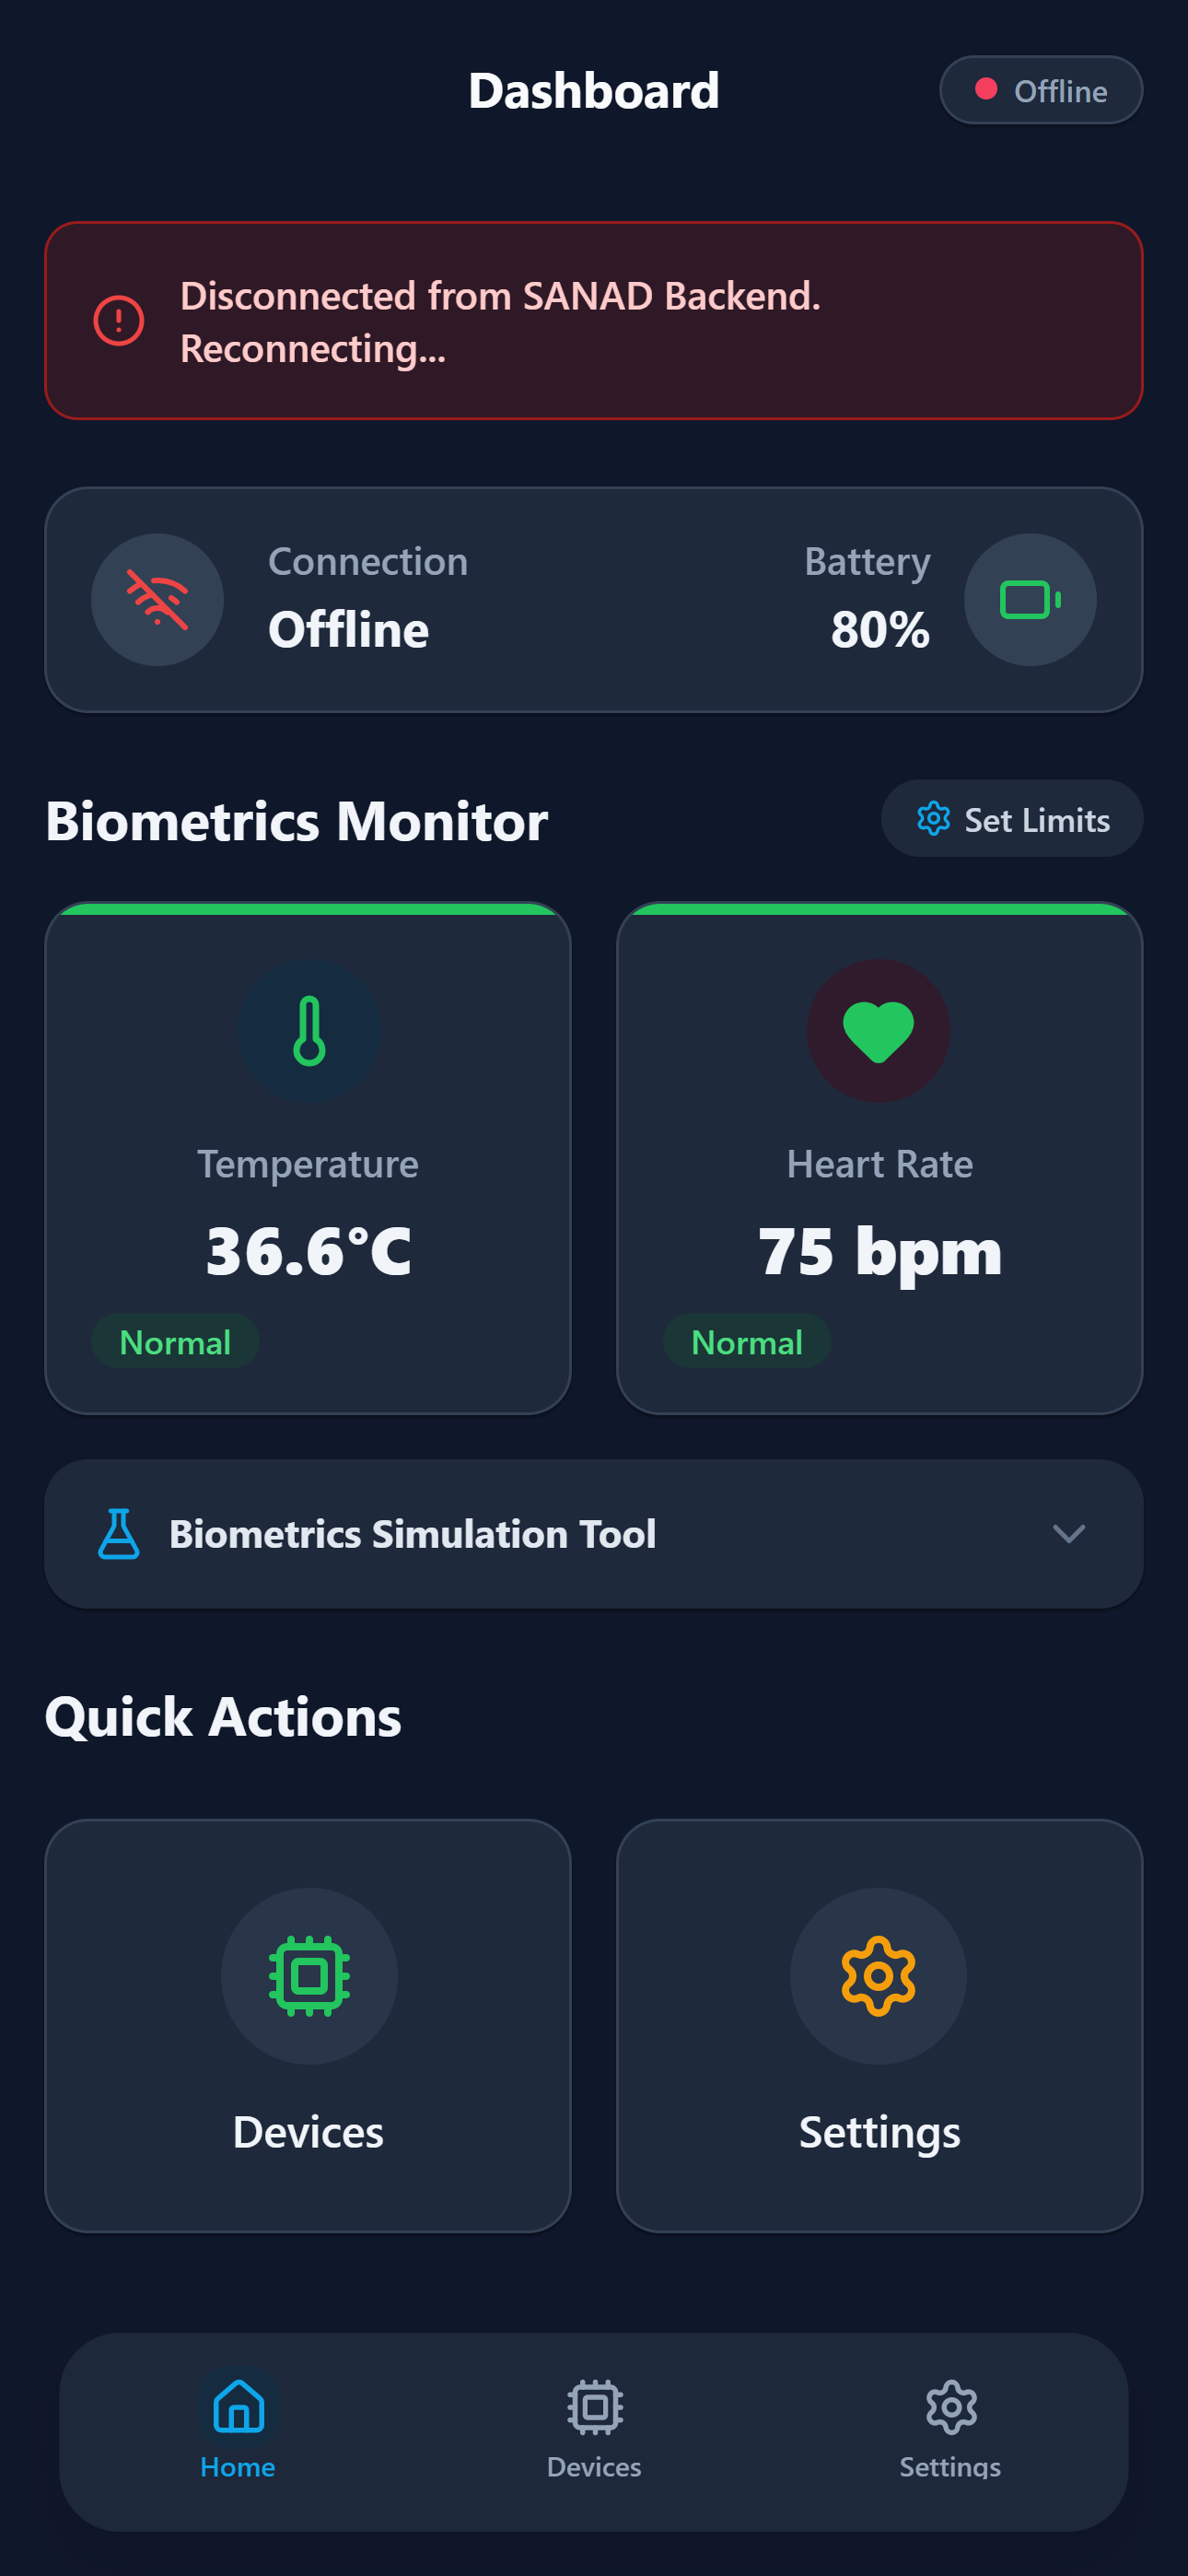
\includegraphics[width=0.48\textwidth]{figures/ch09/biometrics_cards.png}
\caption{Real-time Biometrics dashboard cards showing temperature and heart rate metrics with status badges.}
\label{fig:biometrics-cards}
\end{figure}

\section{Telegram Alert Integration \& Destination Matching}
To deliver alerts even when the mobile app is closed, the system integrates with the Telegram Bot API. 

When the biometrics monitor detects a threshold breach, it dispatches the alert message using the Telegram service wrapper. The backend bot then forwards the alert to the selected recipient. Caregivers can configure the alert destination in the settings panel, choosing between:
\begin{itemize}
    \item \textbf{Saved Messages (Me)}: Sends alerts directly to the caregiver's personal Telegram chat.
    \item \textbf{Group Dialogs}: Sends alerts to a shared family or medical Telegram group.
\end{itemize}

The list of available chats is fetched from the Telegram client API using the user's ID by querying the registered users and groups endpoints on the backend. The selected chat ID is saved locally on the device using \texttt{AsyncStorage} under the key \texttt{"@sannad\_biometric\_target\_chat"}. This ensures alert routing preferences persist across app restarts.

\begin{figure}[H]
\centering
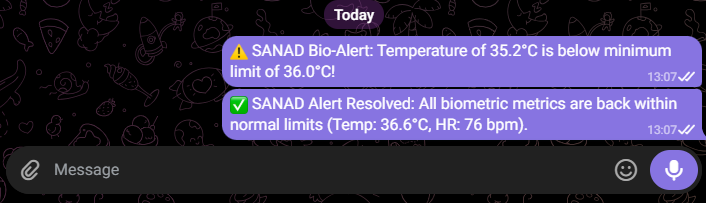
\includegraphics[width=0.5\textwidth]{figures/ch09/telegram_alert_msg.png}
\caption{Caregiver's phone screen showing a real-time emergency alert message received via the Telegram Bot.}
\label{fig:telegram-alert-msg}
\end{figure}

\section{Smart Home \& Device Discovery}
The Smart Home view (\texttt{smart-home.tsx}) allows caregivers to control IoT devices in the patient's room from their mobile phone.

Discovered smart devices are grouped and displayed by room. Caregivers can toggle devices (like lights and TVs) using switch widgets. If no devices are detected, the app displays an empty state illustration with a "Discover Devices" button. Clicking this sends a scan request to the server, which runs a UDP broadcast to discover active devices and update the local list.

\begin{figure}[H]
\centering
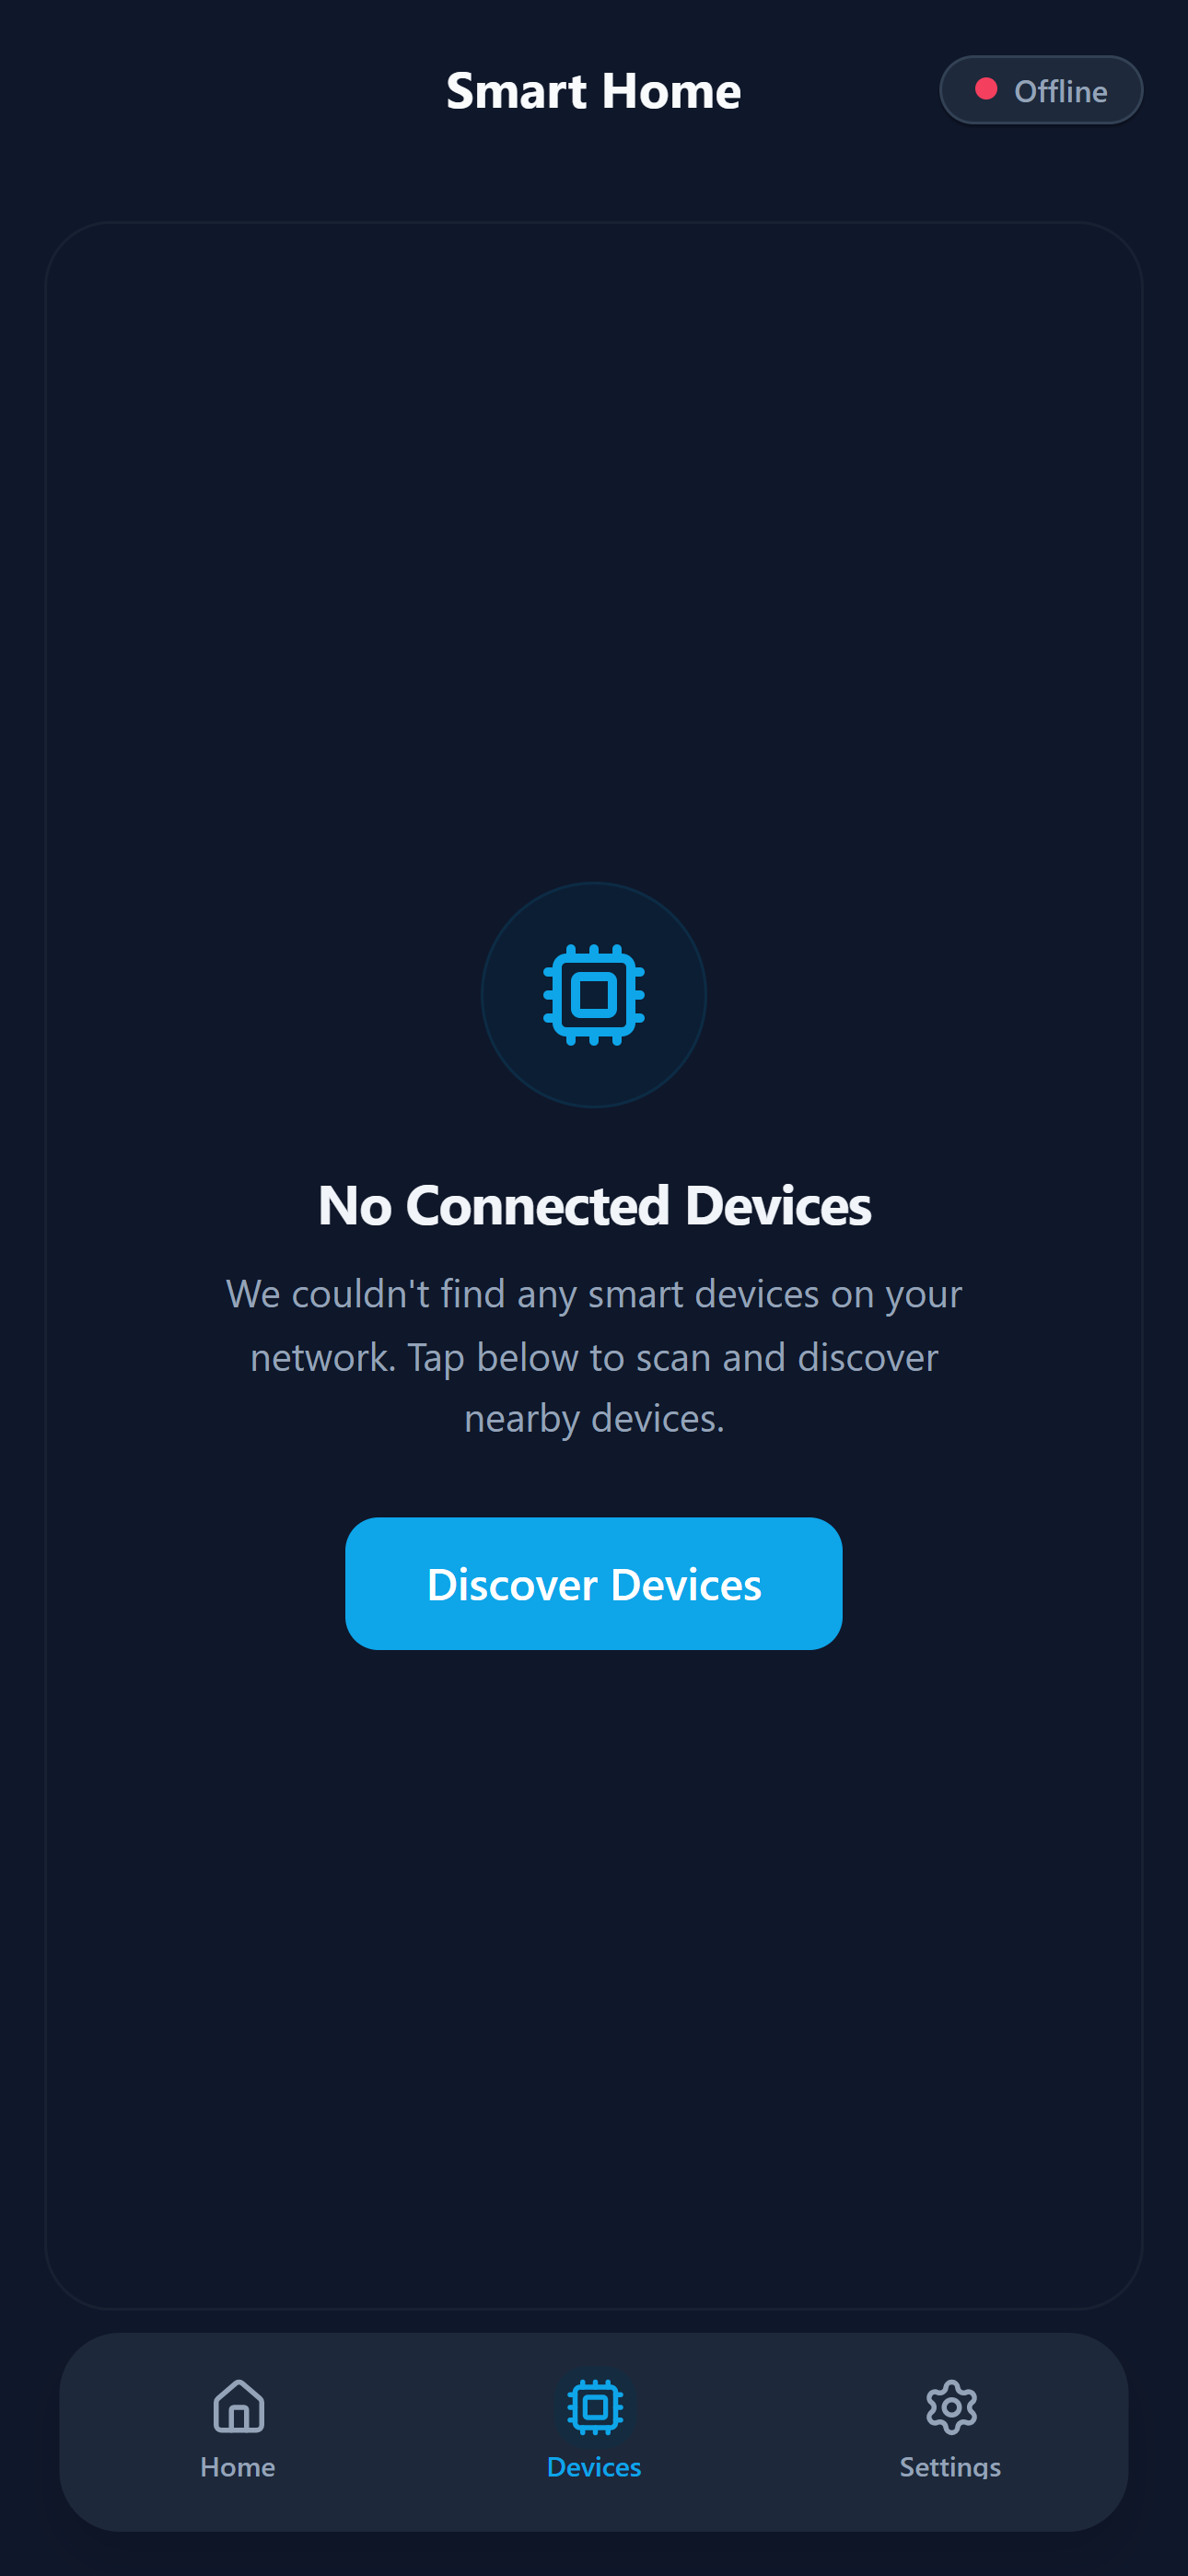
\includegraphics[width=0.45\textwidth]{figures/ch09/mobile_smarthome.png}
\caption{Smart Home control tab showing connected appliances categorized by their assigned room.}
\label{fig:mobile-smarthome}
\end{figure}

\section{Authentication \& Telegram OTP Verification}
To secure access to the wheelchair telemetry and controls, caregivers must authenticate when opening the app.

The authentication screen (\texttt{login.tsx}) handles both login and registration. If a user enters an unregistered email, the app transitions to the sign-up form, requesting their name, password, and Telegram phone number. To connect their account with the Telegram bot, the user must complete an OTP (One-Time Password) verification flow:
\begin{itemize}
    \item The app sends the user's phone number to the backend's Telegram session manager.
    \item The backend bot requests a connection code from Telegram's servers.
    \item The user receives a login code via their official Telegram app, which they enter on the mobile app's verification screen.
    \item Once verified, the backend creates a persistent Telegram session string for that user, enabling automated alert notifications.
\end{itemize}

\begin{figure}[H]
\centering
\begin{tikzpicture}[
    font=\sffamily\small,
    scale=0.95
]
    % Lifelines
    \draw[thick, dashed] (0,0) -- (0,-6.5) node[below] {Mobile Client};
    \draw[thick, dashed] (4,0) -- (4,-6.5) node[below] {Node.js Backend};
    \draw[thick, dashed] (8,0) -- (8,-6.5) node[below] {Telegram API};

    % Lifeline Headers
    \node[draw, rectangle, fill=blue!10, minimum width=2.5cm, minimum height=0.6cm] at (0,0.3) {Mobile Client};
    \node[draw, rectangle, fill=orange!10, minimum width=2.5cm, minimum height=0.6cm] at (4,0.3) {Node.js Backend};
    \node[draw, rectangle, fill=cyan!10, minimum width=2.5cm, minimum height=0.6cm] at (8,0.3) {Telegram API};

    % Steps
    \draw[-Latex, thick, draw=blue!80!black] (0,-1) -- node[above, font=\tiny] {1. Send Phone Number} (4,-1);
    \draw[-Latex, thick, draw=orange!80!black] (4,-2) -- node[above, font=\tiny] {2. Request OTP Code} (8,-2);
    \draw[-Latex, dashed, thick, draw=cyan!80!black] (8,-3.5) -- node[above, font=\tiny, align=center] {3. Send OTP Code\\(via Telegram App)} (0,-3.5);
    \draw[-Latex, thick, draw=blue!80!black] (0,-4.5) -- node[above, font=\tiny] {4. Submit Verification OTP} (4,-4.5);
    \draw[-Latex, thick, draw=orange!80!black] (4,-5.2) -- node[above, font=\tiny] {5. Validate \& Fetch Session} (8,-5.2);
    \draw[-Latex, thick, draw=green!60!black] (4,-6) -- node[above, font=\tiny] {6. Authentication Confirmed} (0,-6);

\end{tikzpicture}
\caption{Sequence diagram illustrating the Telegram OTP authentication and persistent session handshake flow.}
\label{fig:mobile-otp-sequence}
\end{figure}

\begin{figure}[H]
\centering
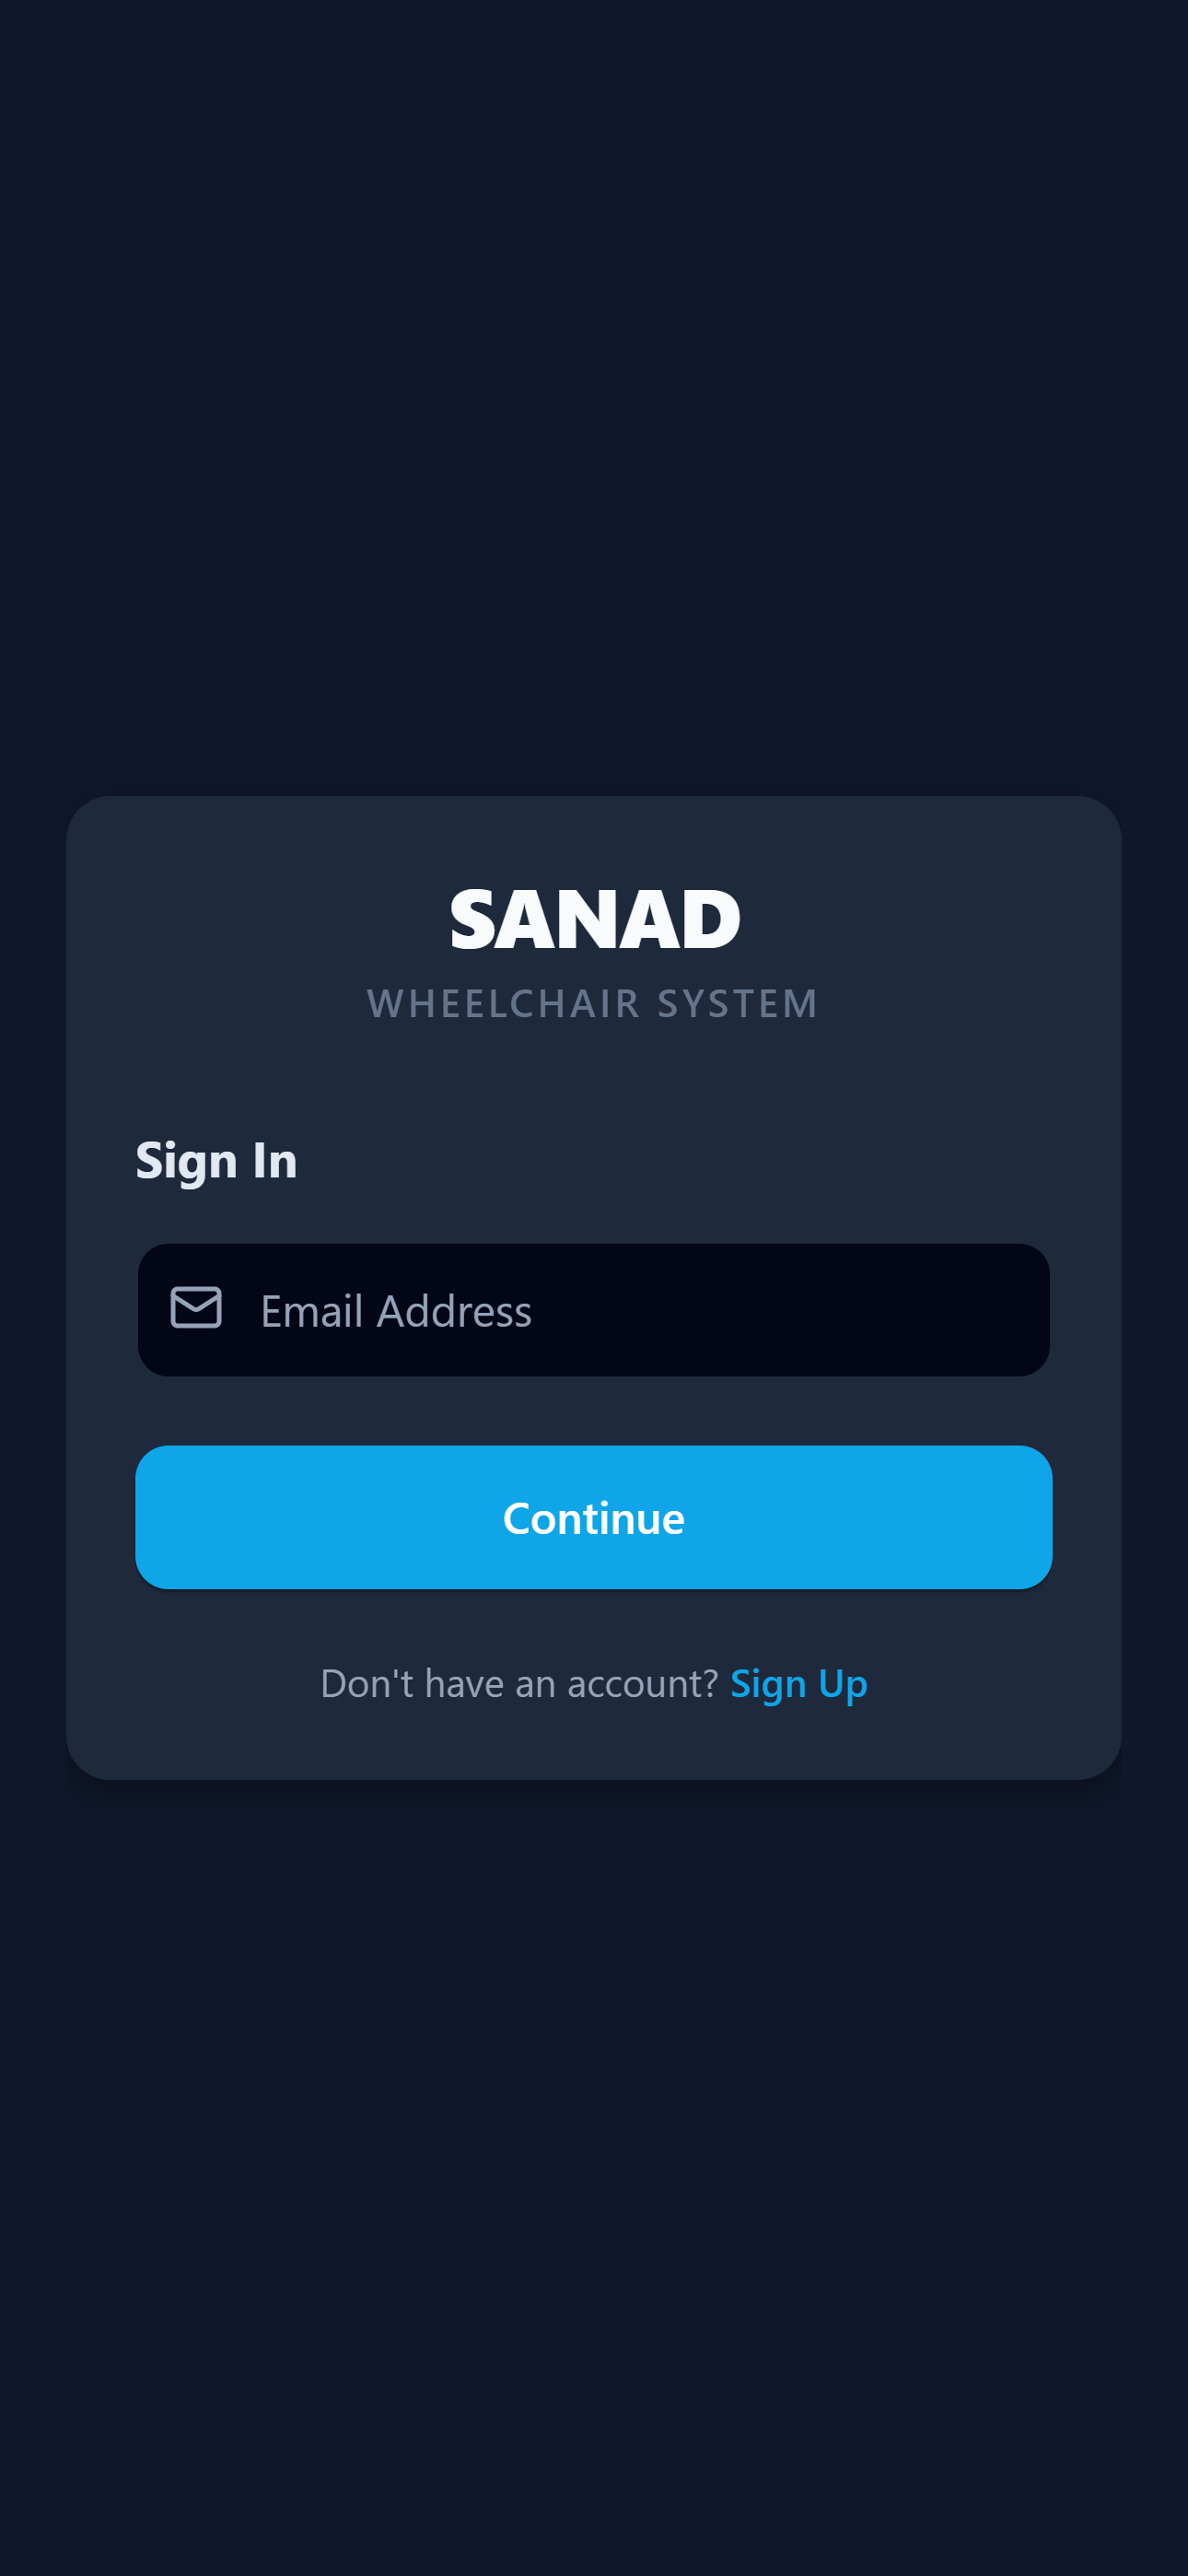
\includegraphics[width=0.48\textwidth]{figures/ch09/mobile_login.png}
\caption{Caregiver login and registration interface in the mobile application.}
\label{fig:mobile-login}
\end{figure}

\begin{figure}[H]
\centering
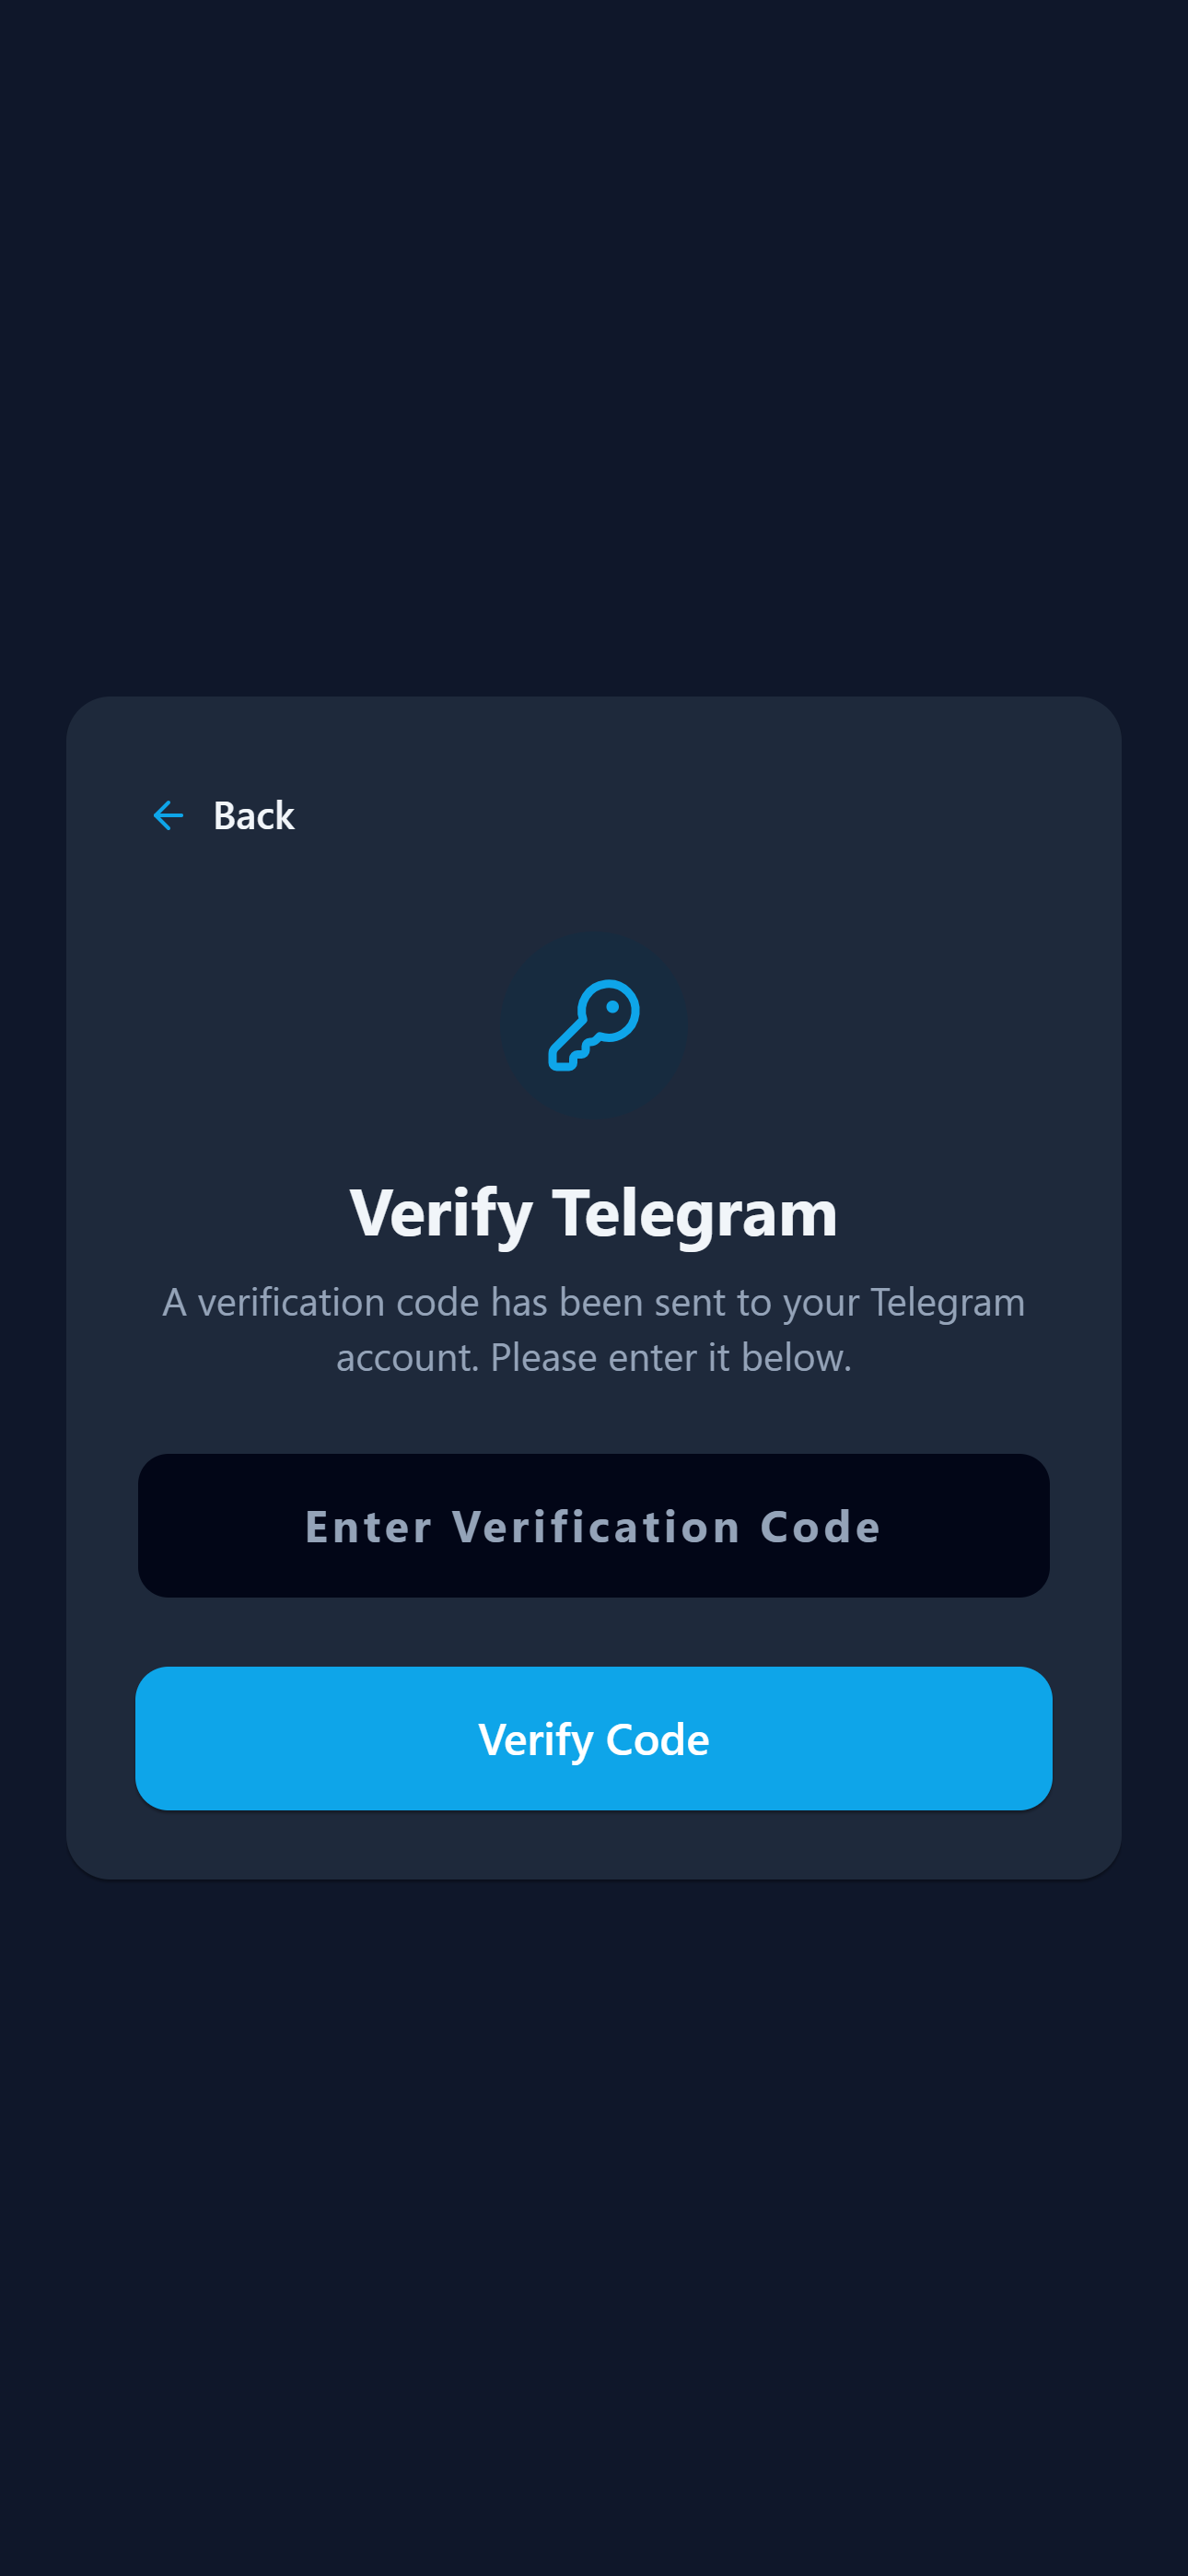
\includegraphics[width=0.48\textwidth]{figures/ch09/mobile_otp.png}
\caption{Telegram OTP Verification screen requesting the authentication code sent to the caregiver's Telegram client.}
\label{fig:mobile-otp}
\end{figure}

\section{Accessibility \& Haptic Feedback}
The mobile app is designed to be accessible to a wide range of users, using physical haptic feedback and accessibility tags to improve usability.

\subsection{Haptic Verification}
To reassure users that their actions and alert thresholds have been updated successfully, the app uses device vibration patterns powered by \texttt{expo-haptics} when saves occur. In addition, the device triggers vibration alerts when emergency alerts are dispatched, helping to draw attention to critical vitals breaches.

\subsection{Accessibility Elements}
The UI is optimized for screen readers (like VoiceOver on iOS and TalkBack on Android). Buttons and interactive elements use semantic labels (\texttt{accessibilityLabel}) and state markers (\texttt{accessibilityState}), and touch targets are sized to at least $48 \times 48$ density-independent pixels to ensure they are easy to select.

\begin{figure}[H]
\centering
\begin{tikzpicture}[
    font=\sffamily\small,
    scale=0.95,
    phone/.style={draw=black!85, thick, fill=gray!3, rounded corners=12pt, minimum width=4.5cm, minimum height=8.0cm},
    card/.style={draw=blue!70!black, fill=white, rounded corners=3pt, minimum width=1.8cm, minimum height=1.5cm, align=center},
    targetZone/.style={draw=red!70, dashed, thick, rounded corners=2pt},
    arrow/.style={-Latex, thin, draw=gray!70}
]

    % Phone Body
    \node[phone] (screen) {};
    
    % Speaker/Camera Notch
    \draw[fill=black!85] (-0.8,3.85) rectangle (0.8,3.65);

    % Screen Header
    \draw[draw=gray!50, fill=gray!15] (-2.1,3.4) rectangle (2.1,2.8);
    \node[font=\tiny\bfseries, text=gray!80!black] at (0,3.1) {Patient Diagnostics Dashboard};
    
    % Card Row 1: Vitals Grid
    \node[card] (hrCard) at (-1.0, 1.8) {\tiny\bfseries Heart Rate\\\tiny 75 bpm};
    \node[card] (tempCard) at (1.0, 1.8) {\tiny\bfseries Temperature\\\tiny 36.6$^\circ$C};
    
    % Dash Touch target zones overlaying cards
    \node[targetZone, fit=(hrCard), inner sep=4pt] (hrTarget) {};
    \node[targetZone, fit=(tempCard), inner sep=4pt] (tempTarget) {};

    % Slider Control Section
    \draw[draw=gray!40, fill=white, rounded corners=3pt] (-2.0, 0.4) rectangle (2.0, -1.2);
    \node[anchor=north west, font=\tiny\bfseries, text=gray!80!black] at (-1.9,0.3) {Threshold Adjuster};
    
    % Slider bar
    \draw[draw=gray!40, fill=gray!20, rounded corners=1pt] (-1.6, -0.4) rectangle (1.6, -0.5);
    \draw[fill=blue!60!black] (-0.3, -0.45) circle (0.15cm);
    
    % Slider Thumb touch target zone
    \node[targetZone, circle, minimum size=0.8cm] (thumbTarget) at (-0.3, -0.45) {};

    % Bottom Navigation Bar
    \draw[draw=gray!50, fill=gray!15] (-2.1,-3.4) rectangle (2.1,-2.7);
    \node[draw=blue!40!black, fill=white, rounded corners=2pt, font=\tiny, inner sep=3pt] (tabHome) at (-1.2, -3.05) {Home};
    \node[font=\tiny, text=gray] (tabSmart) at (0, -3.05) {Devices};
    \node[font=\tiny, text=gray] (tabSet) at (1.2, -3.05) {Settings};
    
    \node[targetZone, fit=(tabHome), inner sep=3pt] (t1) {};
    \node[targetZone, fit=(tabSmart), inner sep=3pt] (t2) {};
    \node[targetZone, fit=(tabSet), inner sep=3pt] (t3) {};

    % Annotations
    \node[anchor=west, font=\tiny, text=red!80!black, align=left] (targetLabel) at (2.8, 0.5) {WCAG 2.1 AA Bounding\\Touch Targets\\($48\text{ dp} \times 48\text{ dp}$ min)};
    
    \draw[arrow] (targetLabel.west) -- (tempTarget.east);
    \draw[arrow] (targetLabel.west) -- (thumbTarget.east);
    \draw[arrow] (targetLabel.west) -- (t3.east);

\end{tikzpicture}
\caption{UX layout wireframe showing dashboard card structure, Flexbox spacing, and accessibility touch target zones (minimum $48 \times 48\text{ dp}$ bounds) for the mobile app interface.}
\label{fig:mobile-wireframe}
\end{figure}

\section{System Diagnostics}
The settings panel (\texttt{settings.tsx}) displays system diagnostic information to help caregivers monitor the wheelchair's status.

When connected to the server, the app subscribes to status topics like battery state and diagnostics. It parses these messages to display:
\begin{itemize}
    \item \textbf{Battery Level}: Extracted from the battery state message percentage.
    \item \textbf{Speed Limit}: The current speed limit setting (0--100\%).
    \item \textbf{System Temperature}: The CPU temperature of the onboard computer.
    \item \textbf{Uptime}: The elapsed time since the system was powered on.
\end{itemize}
This panel also allows caregivers to update the server's API URL when connecting to different local networks.

\begin{figure}[H]
\centering
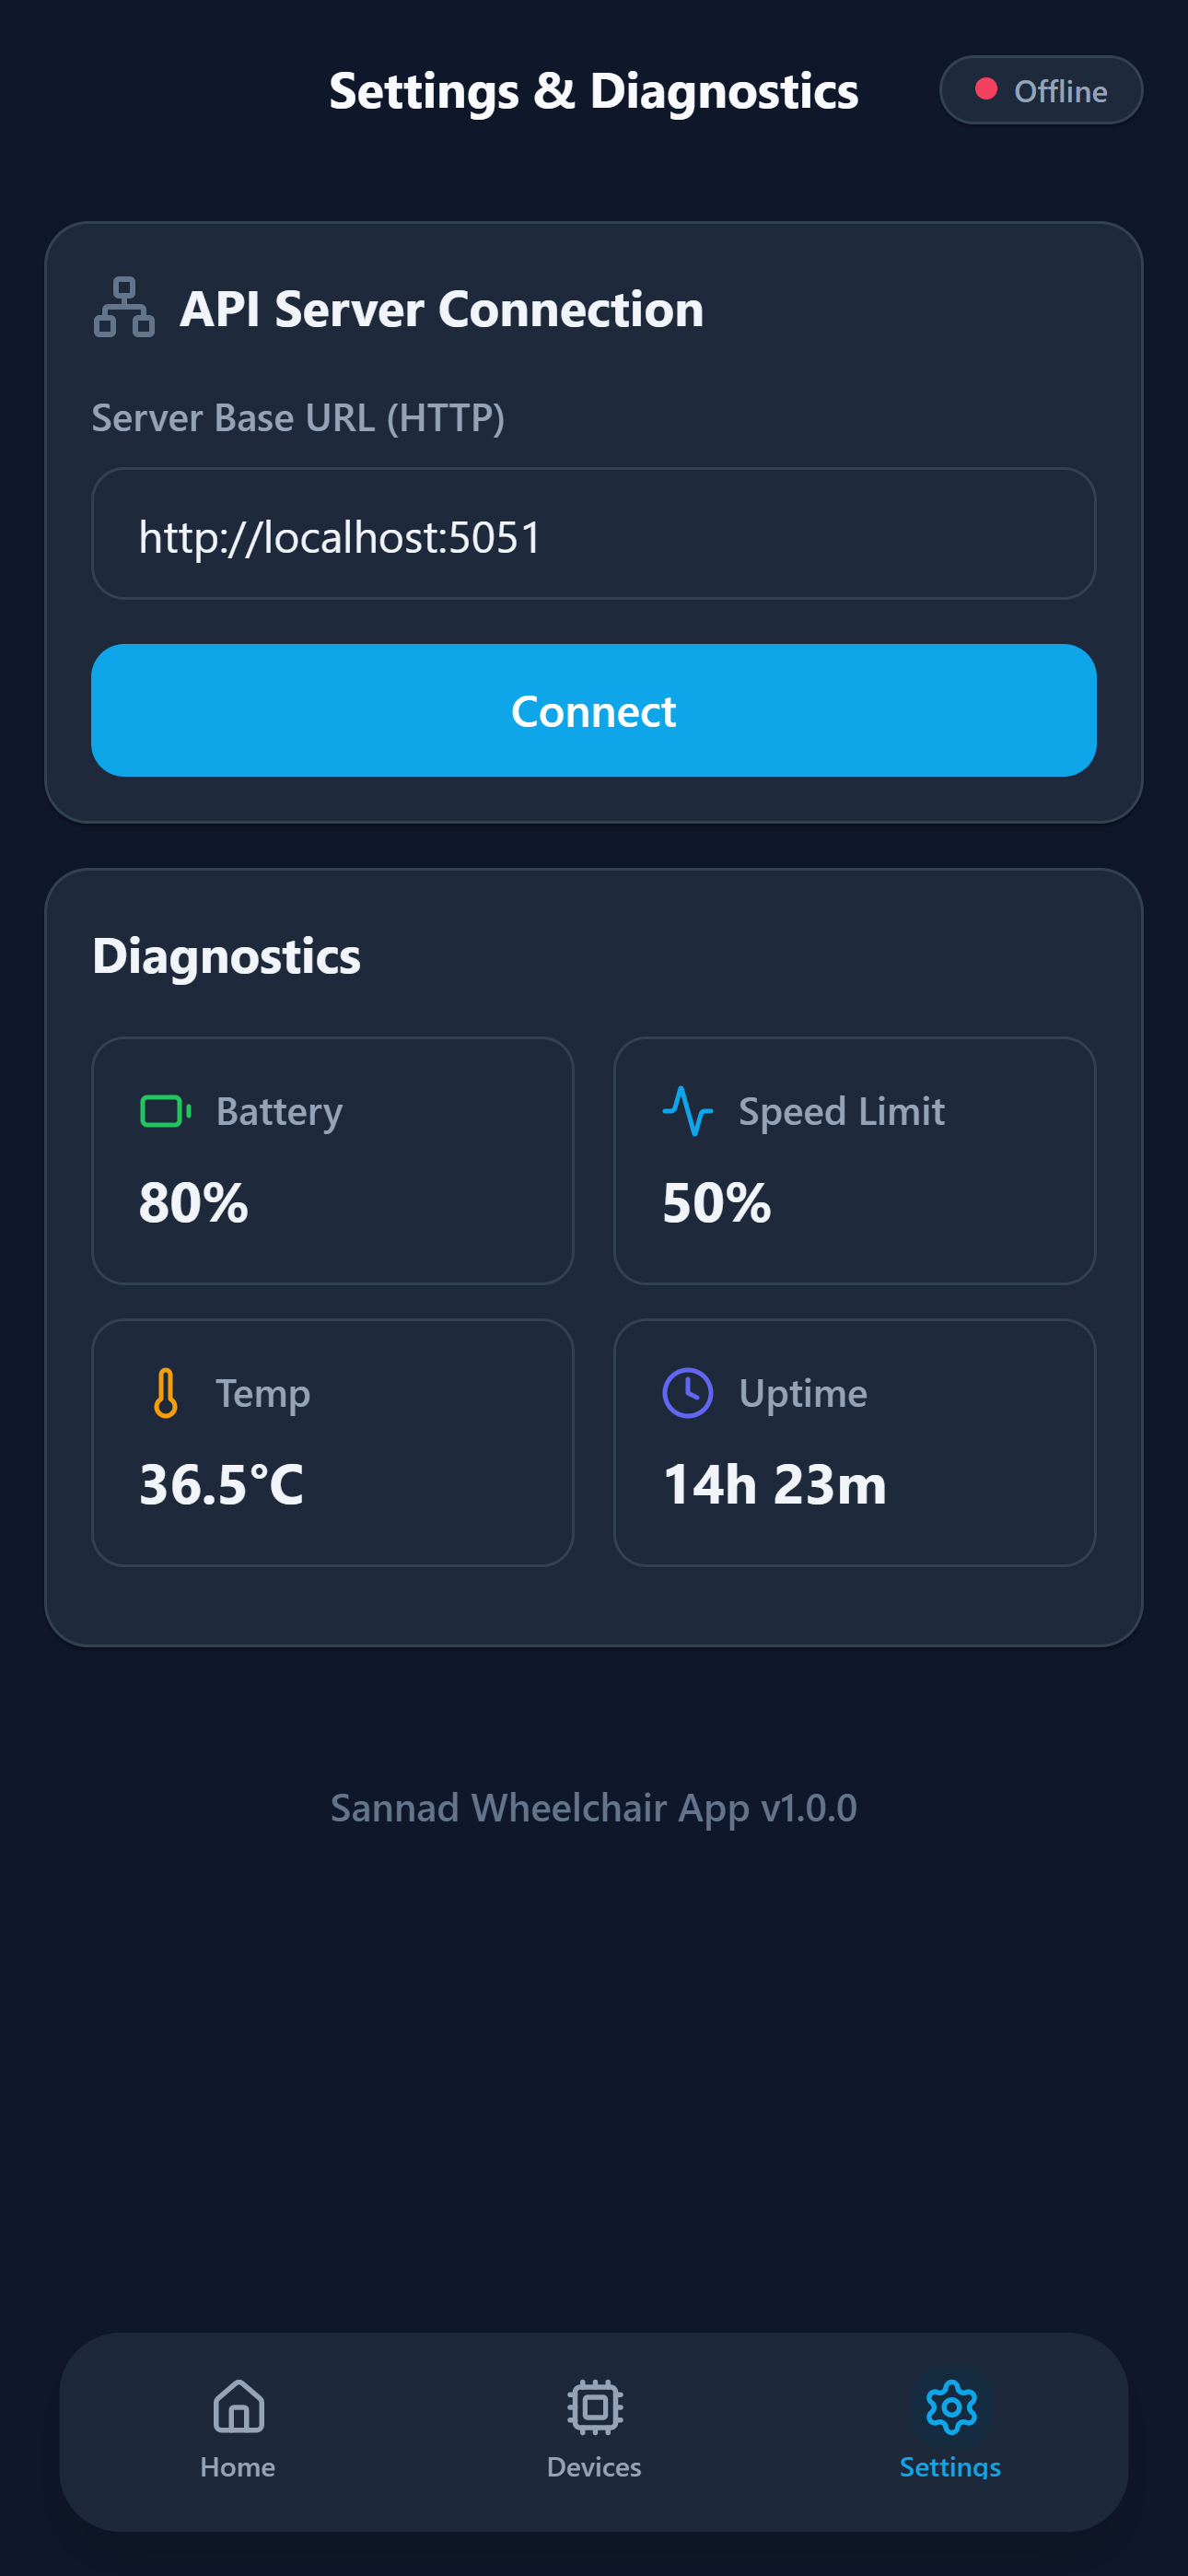
\includegraphics[width=0.45\textwidth]{figures/ch09/mobile_settings.png}
\caption{Settings and Diagnostics view showing server configuration inputs and active wheelchair diagnostic readings.}
\label{fig:mobile-settings}
\end{figure}

\section{Summary and Transition}
This chapter has detailed the design of the React Native mobile app, highlighting caregiver biometrics telemetry and remote system diagnostic capabilities. The next chapter, Chapter 10 (Hardware \& Implementation), focuses on the physical integration, custom circuit layouts, motor control loops, and power configurations of the wheelchair.
